%\chapter*{Annexes}
%\phantomsection

%\addcontentsline{toc}{chapter}{Annexes}

\phantomsection
\addcontentsline{toc}{subsection}{Acoustics of Tube Models}
\thispagestyle{empty}

{\LARGE \textbf{Acoustics of Tube Models (2):\\ Kelly and Lochbaum method}}\label{atm}

\subsection*{1. \textit{n}-section models of the vocal tract}

The actual profile of the vocal tract bears little resemblance to the two-tube models considered in the previous lecture. For example, figure \ref{f1} shows the actual volume profile of a male speaker's vocal tract articulating the vowel {[}\ae {]}. (The figure is computed from MRI scans, and was obtained from \href{https://slhs.arizona.edu/person/brad-story-phd}{Brad Story's website.})

\captionsetup[figure]{list=no}
\setcounter{figure}{0}
\makeatletter 
\renewcommand{\thefigure}{\@arabic\c@figure}
\makeatother

\begin{figure}[htbp]
\begin{center}
%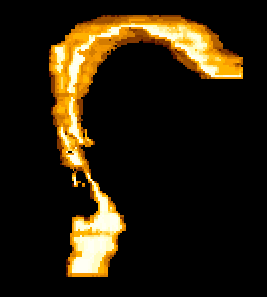
\includegraphics[width=0.5\textwidth]{mp/img/male-ae.png}
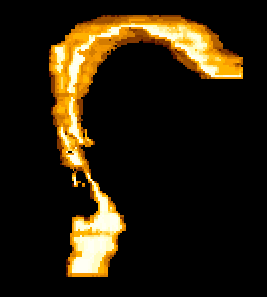
\includegraphics[width=0.45\textwidth]{mp/img/male-ae.png}
\caption{Vocal tract profile of {[}\ae {]}.}
\label{f1}
\end{center}
\end{figure}

%\newpage 

\begin{figure}[htbp]
\begin{center}
%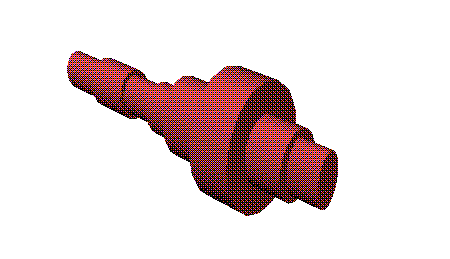
\includegraphics[width=0.7\textwidth]{mp/img/eight-section-model.png}
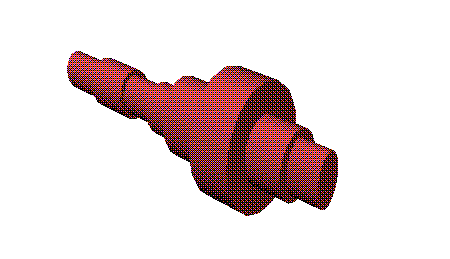
\includegraphics[width=0.65\textwidth]{mp/img/eight-section-model.png}
\caption{Eight section tube model of vocal tract.}
\label{f2}
\end{center}
\end{figure}

\newpage

In an attempt to model such profiles more accurately, we can examine the resonances of many concatenated tubes. Figure \ref{f2} shows an arrangement of eight tubular sections, and figure \ref{f3} the area function of that model:

\begin{figure}[htbp]
\begin{center}
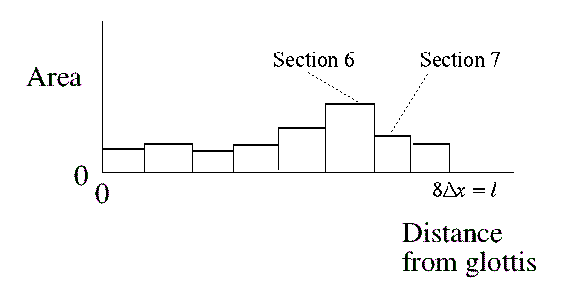
\includegraphics[width=0.7\textwidth]{mp/img/eight-areas.png}
\caption{Pressure waves in a 2-section model.}
\label{f3}
\end{center}
\end{figure}

\vspace{-6mm}

\subsection*{2. Pressure waves in a 2-section model}

We consider the transmission of a wave travelling from the glottis to the lips. Also, because of the steps in the area function, some of the energy is reflected back down the vocal tract. There is also a net `echo', a wave travelling from the lips back to the glottis. Consequently, the pressure \textit{P} in any section is considered to be made up of two components, a forward wave \textit{P\textsuperscript{+}} and a backward wave \textit{P}\textsuperscript{-} (figure \ref{f4}). Thus, \textit{P = P\textsuperscript{+} +P}\textsuperscript{-}.

%\newpage

\begin{figure}[htbp]
\begin{center}
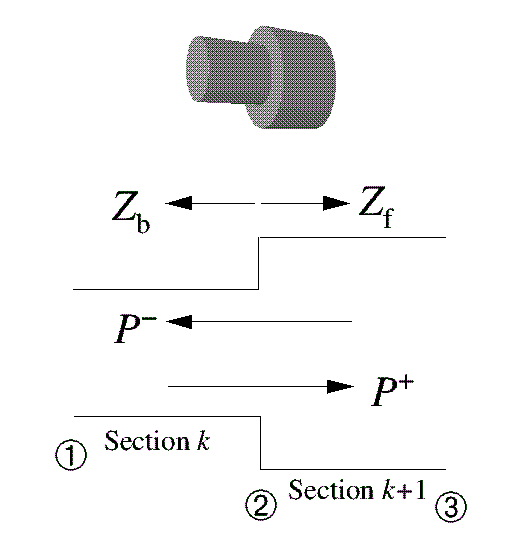
\includegraphics[width=0.55\textwidth]{mp/img/section-interface.png}
\caption{The interface of two tube sections.}
\label{f4}
\end{center}
\end{figure}

Consider what happens at the interface between one tube section and the next (e.g. sections 6 and 7 in figure \ref{f3}). Each tube section has a characteristic impedance (akin to a resistance to airflow). In figure \ref{f4} the impedance forward of the interface (point 2) is labelled \textit{Z}\textsubscript{f} and the impedance of the section behind the interface is labelled \textit{Z}\textsubscript{b}. The forward wave is partly propagated and partly reflected. The reflected fraction \textit{rP\textsuperscript{+}} now becomes part of the backward wave, and the propagated part continues forward. The factor \textit{r} is called the reflection coefficient, and is defined as:

\bigskip

(1)~~~ \textit{r} = (\textit{Z}\textsubscript{f} - \textit{Z}\textsubscript{b})/(\textit{Z}\textsubscript{f} + \textit{Z}\textsubscript{b})

\bigskip

Note that \textit{r} is between -1 and 1. At the interface, \textit{P\textsuperscript{+}} is continuous, hence the propagated fraction must be (1+\textit{r})\textit{P\textsuperscript{+}}, so that:

\bigskip

(2)~~~ \textit{P\textsuperscript{+}} = (1+\textit{r})\textit{P\textsuperscript{+}} - \textit{rP\textsuperscript{+}.}

\bigskip

Exactly similar considerations apply to the backward wave \textit{P}\textsuperscript{-}, except that since it travels in the opposite direction \textit{Z}\textsubscript{f} and \textit{Z}\textsubscript{b} are reversed. Thus the reflection coefficient to the backward wave is:

\bigskip

(3)~~~ (\textit{Z}\textsubscript{b} - \textit{Z}\textsubscript{f})/(\textit{Z}\textsubscript{b} + \textit{Z}\textsubscript{f}) = -\textit{r}

\bigskip

The propagated part of \textit{P}\textsuperscript{-} is therefore (1-\textit{r})\textit{P\textsuperscript{-}}, and the reflected part is -\textit{rP}\textsuperscript{-}. In this case the reflected fraction adds to the forward going wave. This situation is illustrated in figure \ref{f5}:\\

\begin{figure}[htbp]
\begin{center}
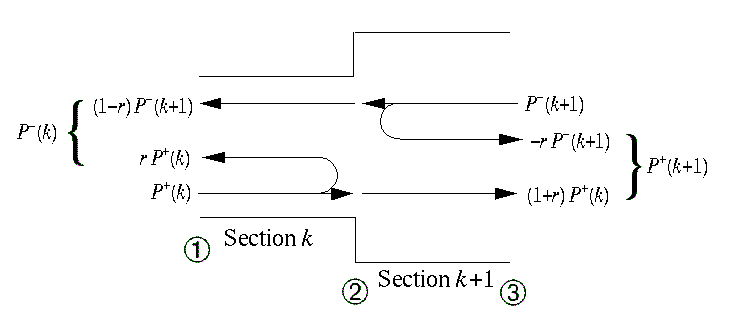
\includegraphics[width=\textwidth]{mp/img/reflections.png}
\caption{Reflection relationships at an abrupt discontinuity in an acoustic tube.}
\label{f5}
\end{center}
\end{figure}


If there are no losses in the tube the acoustic impedances \textit{Z}\textsubscript{f} and \textit{Z}\textsubscript{b} are simple functions of the cross-sectional area \textit{A}(\textit{x}): \textit{Z}\textsubscript{f} = \textit{DV}/\textit{A}\textsubscript{f} and \textit{Z}\textsubscript{b} = \textit{DV}/\textit{A}\textsubscript{b}, from which we can work out that:

\bigskip

(4)~~~ \textit{r} = (\textit{A}\textsubscript{b} - \textit{A}\textsubscript{f})/(\textit{A}\textsubscript{b} + \textit{A}\textsubscript{f}).

\bigskip

(In practise, we can also obtain the reflection coefficients by using linear prediction software, such as the xwaves program \textit{refcof}.)

\bigskip

\subsection*{3. Pressure waves in an \textit{n}-section model}

In a model with n sections, where there are multiple discontinuities, there will be multiple reflections. It is therefore necessary to consider the pressures at discrete points in time, in other words, to consider the signal digitally. For the tube in figure \ref{f5}, the \textit{P\textsuperscript{+}} wave travelling from left to right will propagate undisturbed from point 1 until it reaches the discontinuity at point 2. Similarly, the backward wave \textit{P\textsuperscript{-}} will propagate from point 3 without reflecting until it gets to point 2. If the tube sections are of the same length, \textit{l}, the time taken for \textit{P\textsuperscript{+}} to go from point 1 to point 2 is equal to the time it takes for \textit{P\textsuperscript{-}} to go from point 3 to point 2, i.e. \textit{T} = \textit{l}/c, where c is the velocity of sound.

\bigskip

Thus the pressure variations at point 2 (and every other point) only need to be calculated at discrete time intervals, multiples of \textit{T}. The sample interval \textit{T} must be less than or equal to half of the highest frequency that it is desired to generate. For speech, the highest frequency of interest is about 6 kHz. Sampling rates of 11025 Hz and 16000 Hz are widely used for medium-quality digital recordings of speech. The sample intervals in these two cases are about 0.000091 s (91 $\mu s$) and 0.000063 s (63 $\mu s$) respectively.

\bigskip

The maximum section length \textit{l} is also dependent on the sampling rate, since \textit{T} = \textit{l}/c. For a sampling rate of 11025 Hz, the maximum section length is 0.03084 m; for a vocal tract of length 0.175 m, a minimum of six tube sections will be required. WIth a sampling rate of 16000 Hz, the maximum section length is 0.02125 m, necessitating nine tube sections in the model.

\bigskip

In order to calculate the pressure at any of the junctions in the tube model (and in particular at the `mouth' end), it is necessary to know the pressure wave at the glottis (the closed end of the tube), expressed as a digital signal at time intervals \textit{T} from 0 until some time later time \textit{nT}, the end of the utterance to be generated. A counter is used to increment \textit{T} to 1, and the forward and backward pressures calculated at each interface, according to the reflection coefficients and the equations given in section 2. This process is repeated over and over again, until \textit{nT} is reached. The forward and backward pressures in each section, will change from sample to sample. The forward wave at the mouth end, e.g. \textit{P\textsuperscript{+}}(9) for a nine-section model, will model the sound wave coming out of the mouth.

\bigskip

\subsection*{References}

\noindent Kelly,~ J. L. Jr. and C. C. Lochbaum (1962) Speech Synthesis. In \textit{Proceedings of the Stockholm Speech Communication Seminar.} Reprinted in J. L. Flanagan and L. R. Rabiner, eds. (1973) \textit{Speech Synthesis.} Stroudsberg, PA: Dowden, Hutchinson and Ross. 127-130.

\bigskip

\noindent Linggard, R. (1985) \textit{Electronic Synthesis of Speech.} Cambridge University Press. 61-4.

\begin{center}\rule{0.5\linewidth}{0.5pt}\end{center}

 \href{http://www.phon.ox.ac.uk/jcoleman/kelly-lochbaum.htm}{\texttt{\footnotesize http://www.phon.ox.ac.uk/jcoleman/kelly-lochbaum.htm}}

\bigskip

See also:

\noindent Smith, Julius O. `Singing Kelly-Lochbaum Vocal Tract', in \textit{Physical Audio Signal Processing}, online book, 2010 edition.

\noindent \href{https://ccrma.stanford.edu/~jos/pasp/Singing\_Kelly\_Lochbaum\_Vocal\_Tract.html}{\texttt{\footnotesize https://ccrma.stanford.edu/$\sim$jos/pasp/Singing\_Kelly\_Lochbaum\_Vocal\_Tract.html}}
